% AER E 361 Mission Report Template
% Spring 2023
% Template created by Yiqi Liang and Professor Matthew Nelson

% Document Configuration DO NOT CHANGE
\documentclass[12 pt]{article}
% --------------------LaTeX Packages---------------------------------
% The following are packages that are used in this report.
% DO NOT CHANGE ANY OF THE FOLLOWING OR YOUR REPORT WILL NOT COMPILE
% -------------------------------------------------------------------

\usepackage{hyperref}
\usepackage{parskip}
\usepackage{titlesec}
\usepackage{titling}
\usepackage{graphicx}
\usepackage{graphviz}
\usepackage[T1]{fontenc}
\usepackage{titlesec, blindtext, color} %for LessIsMore style
\usepackage{tcolorbox} %for references box
\usepackage[hmargin=1in,vmargin=1in]{geometry} % use 1 inch margins
\usepackage{float}
\usepackage{tikz}
\usepackage{svg} % Allows for SVG Vector graphics
\usepackage{textcomp, gensymb} %for degree symbol
\hypersetup{
	colorlinks=true,
	linkcolor=blue,
	urlcolor=cyan,
}
\usepackage{biblatex}
\addbibresource{lab-report-bib.bib}
\usepackage{amsmath}
\usepackage{listings}
\usepackage{multicol}
\usepackage{array}

\usepackage{hologo} %KYR: for \BibTeX
%\usepackage{algpseudocode}
%\usepackage{algorithm}
% This configures items for code listings in the document
\usepackage{xcolor}

\usepackage{fancyhdr} % Headers/Footers
\usepackage{siunitx} % SI units
\usepackage{csquotes} % Display Quote
\usepackage{microtype} % Better line breaks

\definecolor{commentsColor}{rgb}{0.497495, 0.497587, 0.497464}
\definecolor{keywordsColor}{rgb}{0.000000, 0.000000, 0.635294}
\definecolor{stringColor}{rgb}{0.558215, 0.000000, 0.135316}
\definecolor{mygreen}{rgb}{0,0.6,0}
\definecolor{mygray}{rgb}{0.5,0.5,0.5}
\definecolor{mymauve}{rgb}{0.58,0,0.82}

\lstdefinestyle{customc}{
  belowcaptionskip=1\baselineskip,
  breaklines=true,
  frame=L,
  xleftmargin=\parindent,
  language=C,
  showstringspaces=false,
  basicstyle=\footnotesize\ttfamily,
  keywordstyle=\bfseries\color{green!40!black},
  commentstyle=\itshape\color{purple!40!black},
  identifierstyle=\color{blue},
  stringstyle=\color{orange},
 }

 \lstset{ %
  backgroundcolor=\color{white},   % choose the background color; you must add \usepackage{color} or \usepackage{xcolor}
  basicstyle=\footnotesize,        % the size of the fonts that are used for the code
  breakatwhitespace=false,         % sets if automatic breaks should only happen at whitespace
  breaklines=true,                 % sets automatic line breaking
  captionpos=b,                    % sets the caption-position to bottom
  commentstyle=\color{commentsColor}\textit,    % comment style
  deletekeywords={...},            % if you want to delete keywords from the given language
  escapeinside={\%*}{*)},          % if you want to add LaTeX within your code
  extendedchars=true,              % lets you use non-ASCII characters; for 8-bits encodings only, does not work with UTF-8
  frame=tb,	                   	   % adds a frame around the code
  keepspaces=true,                 % keeps spaces in text, useful for keeping indentation of code (possibly needs columns=flexible)
  keywordstyle=\color{keywordsColor}\bfseries,       % keyword style
  language=Python,                 % the language of the code (can be overrided per snippet)
  otherkeywords={*,...},           % if you want to add more keywords to the set
  numbers=left,                    % where to put the line-numbers; possible values are (none, left, right)
  numbersep=8pt,                   % how far the line-numbers are from the code
  numberstyle=\tiny\color{commentsColor}, % the style that is used for the line-numbers
  rulecolor=\color{black},         % if not set, the frame-color may be changed on line-breaks within not-black text (e.g. comments (green here))
  showspaces=false,                % show spaces everywhere adding particular underscores; it overrides 'showstringspaces'
  showstringspaces=false,          % underline spaces within strings only
  showtabs=false,                  % show tabs within strings adding particular underscores
  stepnumber=1,                    % the step between two line-numbers. If it's 1, each line will be numbered
  stringstyle=\color{stringColor}, % string literal style
  tabsize=2,	                   % sets default tabsize to 2 spaces
  title=\lstname,                  % show the filename of files included with \lstinputlisting; also try caption instead of title
  columns=fixed                    % Using fixed column width (for e.g. nice alignment)
}

\lstdefinestyle{customasm}{
  belowcaptionskip=1\baselineskip,
  frame=L,
  xleftmargin=\parindent,
  language=[x86masm]Assembler,
  basicstyle=\footnotesize\ttfamily,
  commentstyle=\itshape\color{purple!40!black},
}

\lstset{escapechar=@,style=customc}

\titlelabel{\thetitle.\quad}

% From here on out you can start editing your document
\newcommand{\subtitle}[1]{%
  \posttitle{%
    \par\end{center}
    \begin{center}\LARGE#1\end{center}
    \vskip0.5em}%
}

\newcommand{\etal}{\textit{et al}., }
\newcommand{\ie}{\textit{i}.\textit{e}., }
\newcommand{\eg}{\textit{e}.\textit{g}., }

% Define the headers and footers
\setlength{\headheight}{70.63135pt}
\geometry{head=70.63135pt, includehead=true, includefoot=true}
\pagestyle{fancy}
\fancyhead{}\fancyfoot{} % clears the headers/footers
\fancyhead[L]{\textbf{AER E 322}}
\fancyhead[C]{\textbf{Aerospace Structures Pre-Laboratory}\\
			  \textbf{Lab 8 Thin-Walled Section and Shear Center}\\
			  Section 4 Group 2\\
			  Matthew Mehrtens\\
			  \today}
\fancyhead[R]{\textbf{Spring 2023}}
\fancyfoot[C]{\thepage}

\begin{document}
\section*{Question 1}
\textit{(\num{30} points) For specimens I and II (Table \ref{tbl:question_1_table} below), derive an expression for the area moment of inertia, $I$, about its neutral axis in terms of $h$, $b$ and $t$.}

\textit{Hint: To derive the expression for $I$ for specimens I and II, you can do one of two ways: (\num{1}) calculate $I$ for the horizontal flanges and vertical web individually and then sum up or (\num{2}) use ``subtraction'' method by calculating $I$ for a larger ``outer'' rectangular area and then subtracting it from $I$ of the smaller ``inner'' area. You will also need parallel axis theorem. Also, as indicated in Figure \ref{fig:question_2_fig}, the shear center offset $e$ for the C-channel beams is measured from the center of the vertical web, while $e$ for the circular open-channel pipes is measured from the center of circular cross section. Likewise, height $h$ is measured between mid-planes of top and bottom flanges, and $r$ is mean radius, \ie $r=\frac{OD-t}{2}$.}

\begin{table}[!htbp]
\caption{Dimensions for the two types of cross sections of specimens.}
\begin{center}
	\begin{tabular}{|c|c|c|c|c|c|c|}
		\hline
		Specimen &Cross section &Height, &Width, &Thickness, &Outer &Opening \\
		ID&type&$h$ (\unit{inch})&$b$ (\unit{inch})&$t$ (\unit{inch})&diameter, &angle, \\
		&&&&&$OD$ (\unit{inch})&$2\theta_0$ (\unit{deg})\\
		\hline
		I&Plastic C-channel&2.43&1.456&0.08&N/A&N/A\\
		\hline
		II&Metal C-channel&0.84&0.56&0.055&N/A&N/A\\
		\hline
		III&PVC circular open&N/A&N/A&0.071&1.66&3.1\\
		\hline
		IV&PVC circular open&N/A&N/A&0.071&1.66&36.3\\
		\hline
		V&PVC circular open&N/A&N/A&0.071&1.66&103.7\\
		\hline
	\end{tabular}
\end{center}
\label{tbl:question_1_table}
\end{table}

\textbf{Solution:}

Let the $x$-$y$ axis be centered at the center of the vertical flange. The neutral axis of a symmetrical C-channel is on the horizontal $x$-axis. The moment of inertia, $I$, about the neutral axis can be calculated by finding the moment of inertia for each component (the two horizontal rectangles and a vertical rectangle) and then adding them together. The moment of inertia for a rectangle is shown in Equation \ref{eqn:moment_of_inertia}. Since the centroid of the two horizontal rectangles does not intersect the centroid of the beam, we must use the parallel axis theorem, noted in Equation \ref{eqn:parallel_axis_theorem}.
\begin{align}
	I_\text{rect}&=\frac{1}{12}bh^3\label{eqn:moment_of_inertia}\\
	I&=I_\text{shape}+Ay^2\label{eqn:parallel_axis_theorem}
\end{align}
where $A$ is the area of the shape and $y$ is the distance from the centroid of the shape to the neutral axis.

Using these formulas, we can calculate the moment of inertia, $I$, for the C-channel beam as shown below:
\begin{align*}
	I&=I_\text{top-rect}+I_\text{vert-rect}+I_\text{bot-rect}\\
	I&=\frac{1}{12}bt^3+bt\left(\frac{h}{2}\right)^2+\frac{1}{12}bt^3+bt\left(-\frac{h}{2}\right)^2+\frac{1}{12}t(h-t)^3
\end{align*}
Simplifying the above equation, we find that the general formula for calculating the moment of inertia is Equation \ref{eqn:I}
\begin{align}\label{eqn:I}
	I&=\frac{bt^3}{6}+\frac{bth^2}{2}+\frac{t(h-t)^3}{12}
\end{align}

\section*{Question 2}
\textit{(\num{25} points) Calculate the theoretical shear center of each of the five specimens using the following expressions as derived on pages \numlist{9;11} in lecture notes:}
\begin{align}
	\text{C-channel: }e&=\frac{h^2b^2t}{4I}\label{eqn:c_channel}\\
	\text{Circular open-channel: }e&=\frac{2r[\cos\theta_0(2\pi-2\theta_0)+2\sin\theta_0]}{2\pi-2\theta_0+\sin(2\theta_0)}
\end{align}
\textit{See Figure \ref{fig:question_2_fig} for all the corresponding parameters $h$, $b$, $t$, $r$, and $\theta_0$. Note that the \textcolor{red}{total opening angle is $2\theta_0$}.}

\begin{figure}[htbp]
	\centering
	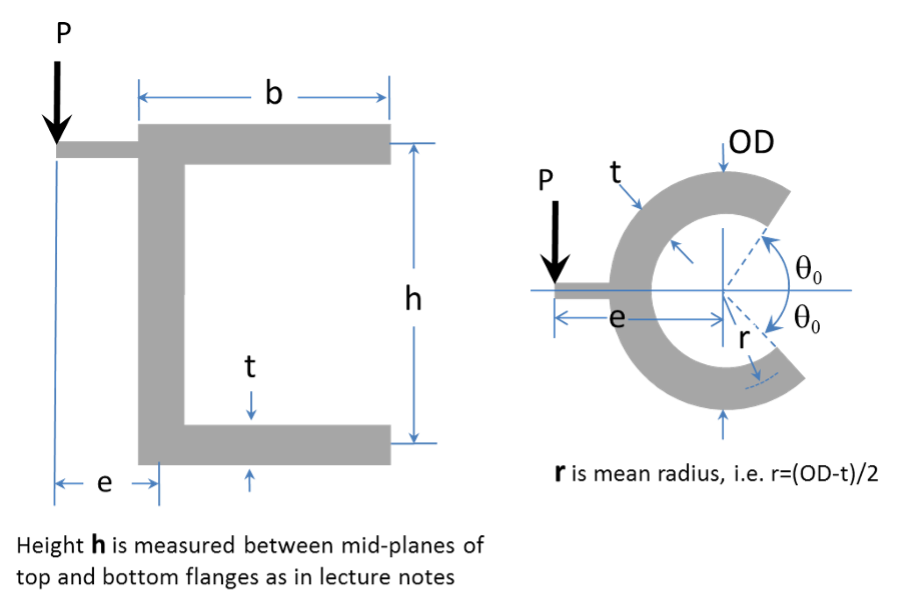
\includegraphics[width=6in]{images/Question 2 Figure}
	\caption{Schematic diagrams of the thin-walled cross section of specimen: (left) C-channel and (right) circular open channel.}
	\label{fig:question_2_fig}
\end{figure}

\textbf{Solution:}

Shear centers are calculated in the MATLAB script attached to this document.

\section*{Question 3}
\textit{(\num{5} points) Tabulate the results.}

\textbf{Solution:}

The results of the previous two questions are tabulated in Table \ref{tbl:question_3_table}.

\begin{table}[!htbp]
\caption{The moments of inertia and shear centers of specimens \num{1}--\num{5}.}
\begin{center}
	\begin{tabular}{|c|c|c|}
		\hline
		Specimen &Moment of Inertia, &Shear Center, \\
		ID&$I$ (\unit{inch^4})&$e$ (\unit{inch})\\
		\hline
		1&\num{0.4305}&\num{0.5815}\\
		\hline
		2&\num{0.01310}&\num{0.2323}\\
		\hline
		3&N/A&\num{1.588}\\
		\hline
		4&N/A&\num{1.507}\\
		\hline
		5&N/A&\num{0.9655}\\
		\hline
	\end{tabular}
\end{center}
\label{tbl:question_3_table}
\end{table}
\end{document}
